\documentclass{article}
\usepackage{graphicx}
\usepackage{caption}
\usepackage{subcaption}
\usepackage[paper=a4paper,margin=1in]{geometry}
\usepackage[fontsize=12pt]{fontsize}
\usepackage{amsmath, amsthm, amssymb}
\usepackage[hidelinks]{hyperref}
\usepackage[nameinlink, noabbrev]{cleveref}

\newtheorem{theorem}{Theorem}[section]
\DeclareMathOperator{\sgn}{sgn}

\title{Math 475 -- Project 2 \\ Stochastic Bobcat Population}
\author{Jackson Brienen}
\date{October 17 2025}

\begin{document}

\maketitle

\section{Introduction}

In this paper we discuss how we can model bobcat populations using stochastic models. We study three different models, one being the basic exponential model, and two being different stochastic models. We approach the models with the following assumptions:

\begin{enumerate}
    \item Any initial population, denoted $P(0)$ will be greater than zero, usually $P(0)=100$.
    \item There is no carrying capacity/ maximum population.
    \item All births and deaths happen at the end of a year/ start of a new year.
    \item All time increments, denoted $t$, are integers greater than or equal to zero.
    \item We assume, in most cases, that fractional populations are valid.
\end{enumerate}

This paper is divided into three main topics. First, a review of the standard exponential population model. Next, a look at demographic stochasticity, i.e. variability in internal growth rates. Finally, we look at environmental stochasticity, which is variability in external factors which will affect population growth.

\section{Exponential Model}

The basic exponential model for bobcat population usually written as \cref{eq:exponential-basic}, focuses primarily on a growth rate $r$. We can expand this parameter to be more realistic, including a birth rate, $b$, and survival rate, $s$. Where $1 + r = b + s$, this creates the more realistic model in \cref{eq:exponential}.

\begin{equation} \label{eq:exponential-basic}
    P(t) = (1 + r)P(t-1)
\end{equation}

\begin{equation} \label{eq:exponential}
    P(t) = (b+s)P(t-1)
\end{equation}

We know that this recurrence simplifies to the exponential function $(r + 1)^tP(0)$, and with our added parameters $(b + s)^tP(0)$. We see this exponential nature in \cref{fig:exponential}. Furthermore, we also see the expected exponential growth as if $b=0.4$ and $s=0.68$, then $s+b = 1.08$. This is the equivalent of having $r = 0.08$ in our simpler formula, which is a positive growth rate.

\begin{figure}
    \centering
    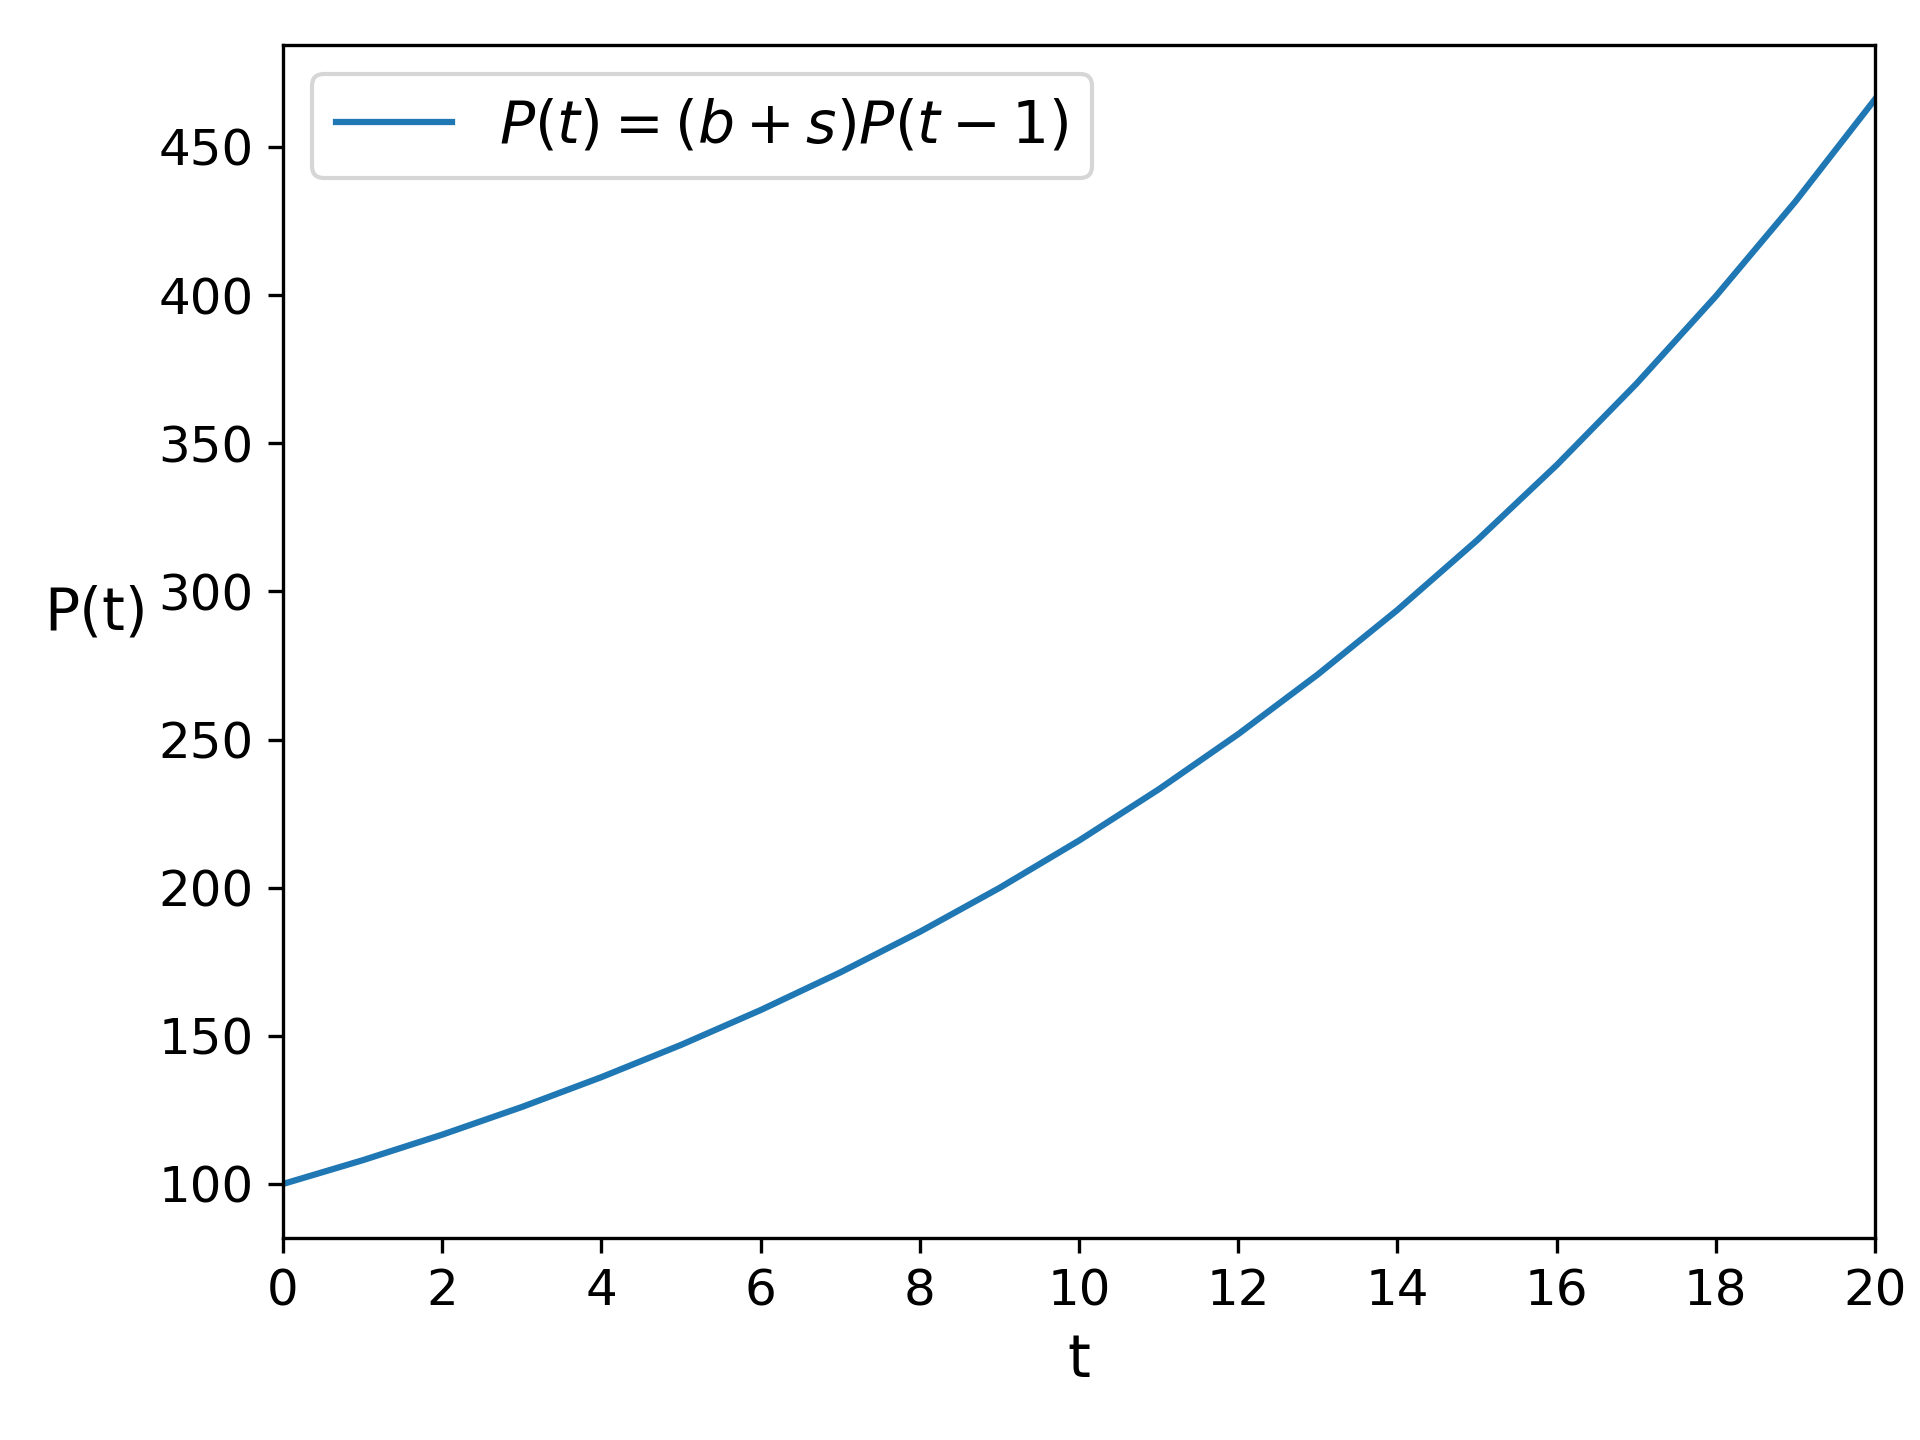
\includegraphics[width=.5\linewidth]{plots/exponential.png}
    \caption{Bobcat population over 20 years with an initial population $P(0)=100$, birth rate $b=0.4$, and survival rate $s=0.68$.}
    \label{fig:exponential}
\end{figure}

\section{Demographic Stochasticity}
While the basic exponential model gives us a good start, it is not very realistic. A constant birth and survival rate is unlikely to happen in real life, so we can attempt to mimic this using demographic stochasticity. Previously our model was deterministic, i.e. the results that we see in \cref{fig:exponential} with the given parameters, will always be the results for those parameters. In a stochastic model we will have parameters that rely on randomness, so using the same model twice may give different results.

For demographic stochasticity we introduce randomness on the two internal parameters, the birth and survival rates. To introduce this randomness we will use a normal distribution. Commonly denoted $z \sim \mathcal{N}(\mu, \sigma)$, where $\mu$ is the mean and $\sigma$ is the standard deviation. The formula for the probability density, seen in \cref{eq:standard-distribution}, describes the general likelihood of a given value, $x$, being chosen.

\begin{equation} \label{eq:standard-distribution}
    f(x) = \frac{1}{\sigma\sqrt{2\pi}}e^{-\frac{1}{2}\left(\frac{x-\mu}{\sigma}\right)^2}
\end{equation}

\begin{figure}[h!]
    \centering
    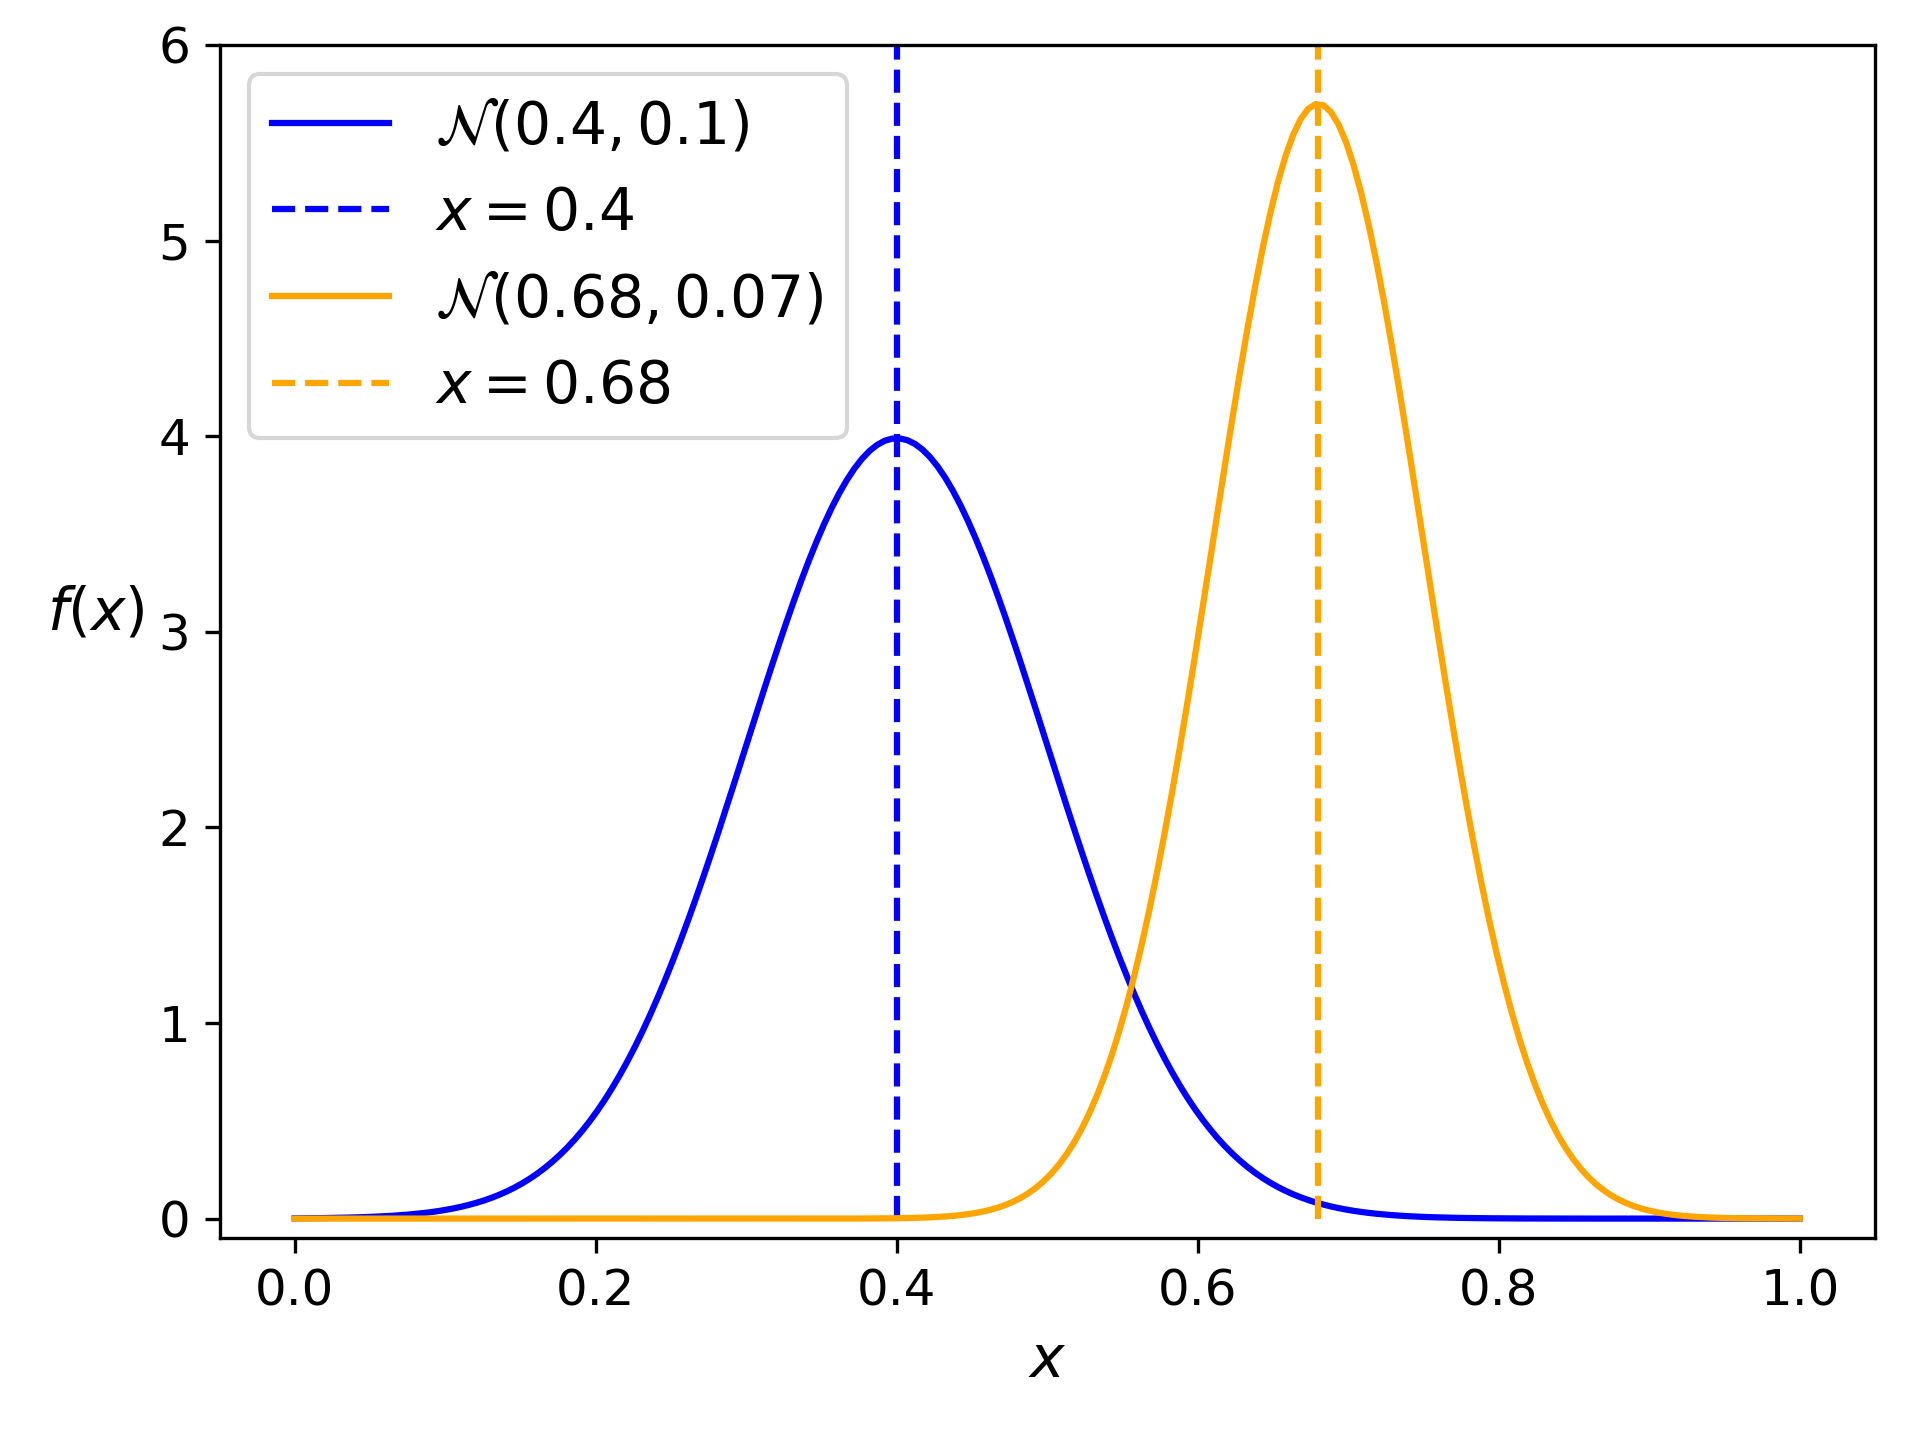
\includegraphics[width=.5\linewidth]{plots/standard-distribution.png}
    \caption{Probability density of standard distributions with means of 0.4 and 0.68, and standard deviations 0.1 and 0.07.}
    \label{fig:standard-distribution}
\end{figure}

Looking at the standard distribution probability densities in \cref{fig:standard-distribution}, we can get a sense of what the standard distribution does. The area under any given region of a curve is the percent chance for those values to be picked, while the area under the whole curve will always be 1 (100\%), provided $\sigma > 0$. In \cref{fig:standard-distribution} we plot $\mathcal{N}(0.4, 0.1)$, the blue line, and $\mathcal{N}(0.68, 0.07)$, the orange line, which will be the distributions we will use for our $b$ and $s$ parameters respectively.

When analyzing this model, due to its inherent randomness, we must take multiple samples or trial runs. We will analyze three components of the model, the maximum population produced, the minimum population produced, and the median population produced. We will compare each of these to the standard deterministic model. It does not make sense to analyze the average population produced by the model. Due to how the normal distribution works, as trial runs increase, the closer the model's average will get to the deterministic model regardless of the standard deviation for the two parameters.

\begin{figure}[h]
    \centering
    \begin{subfigure}{.5\textwidth}
        \centering
        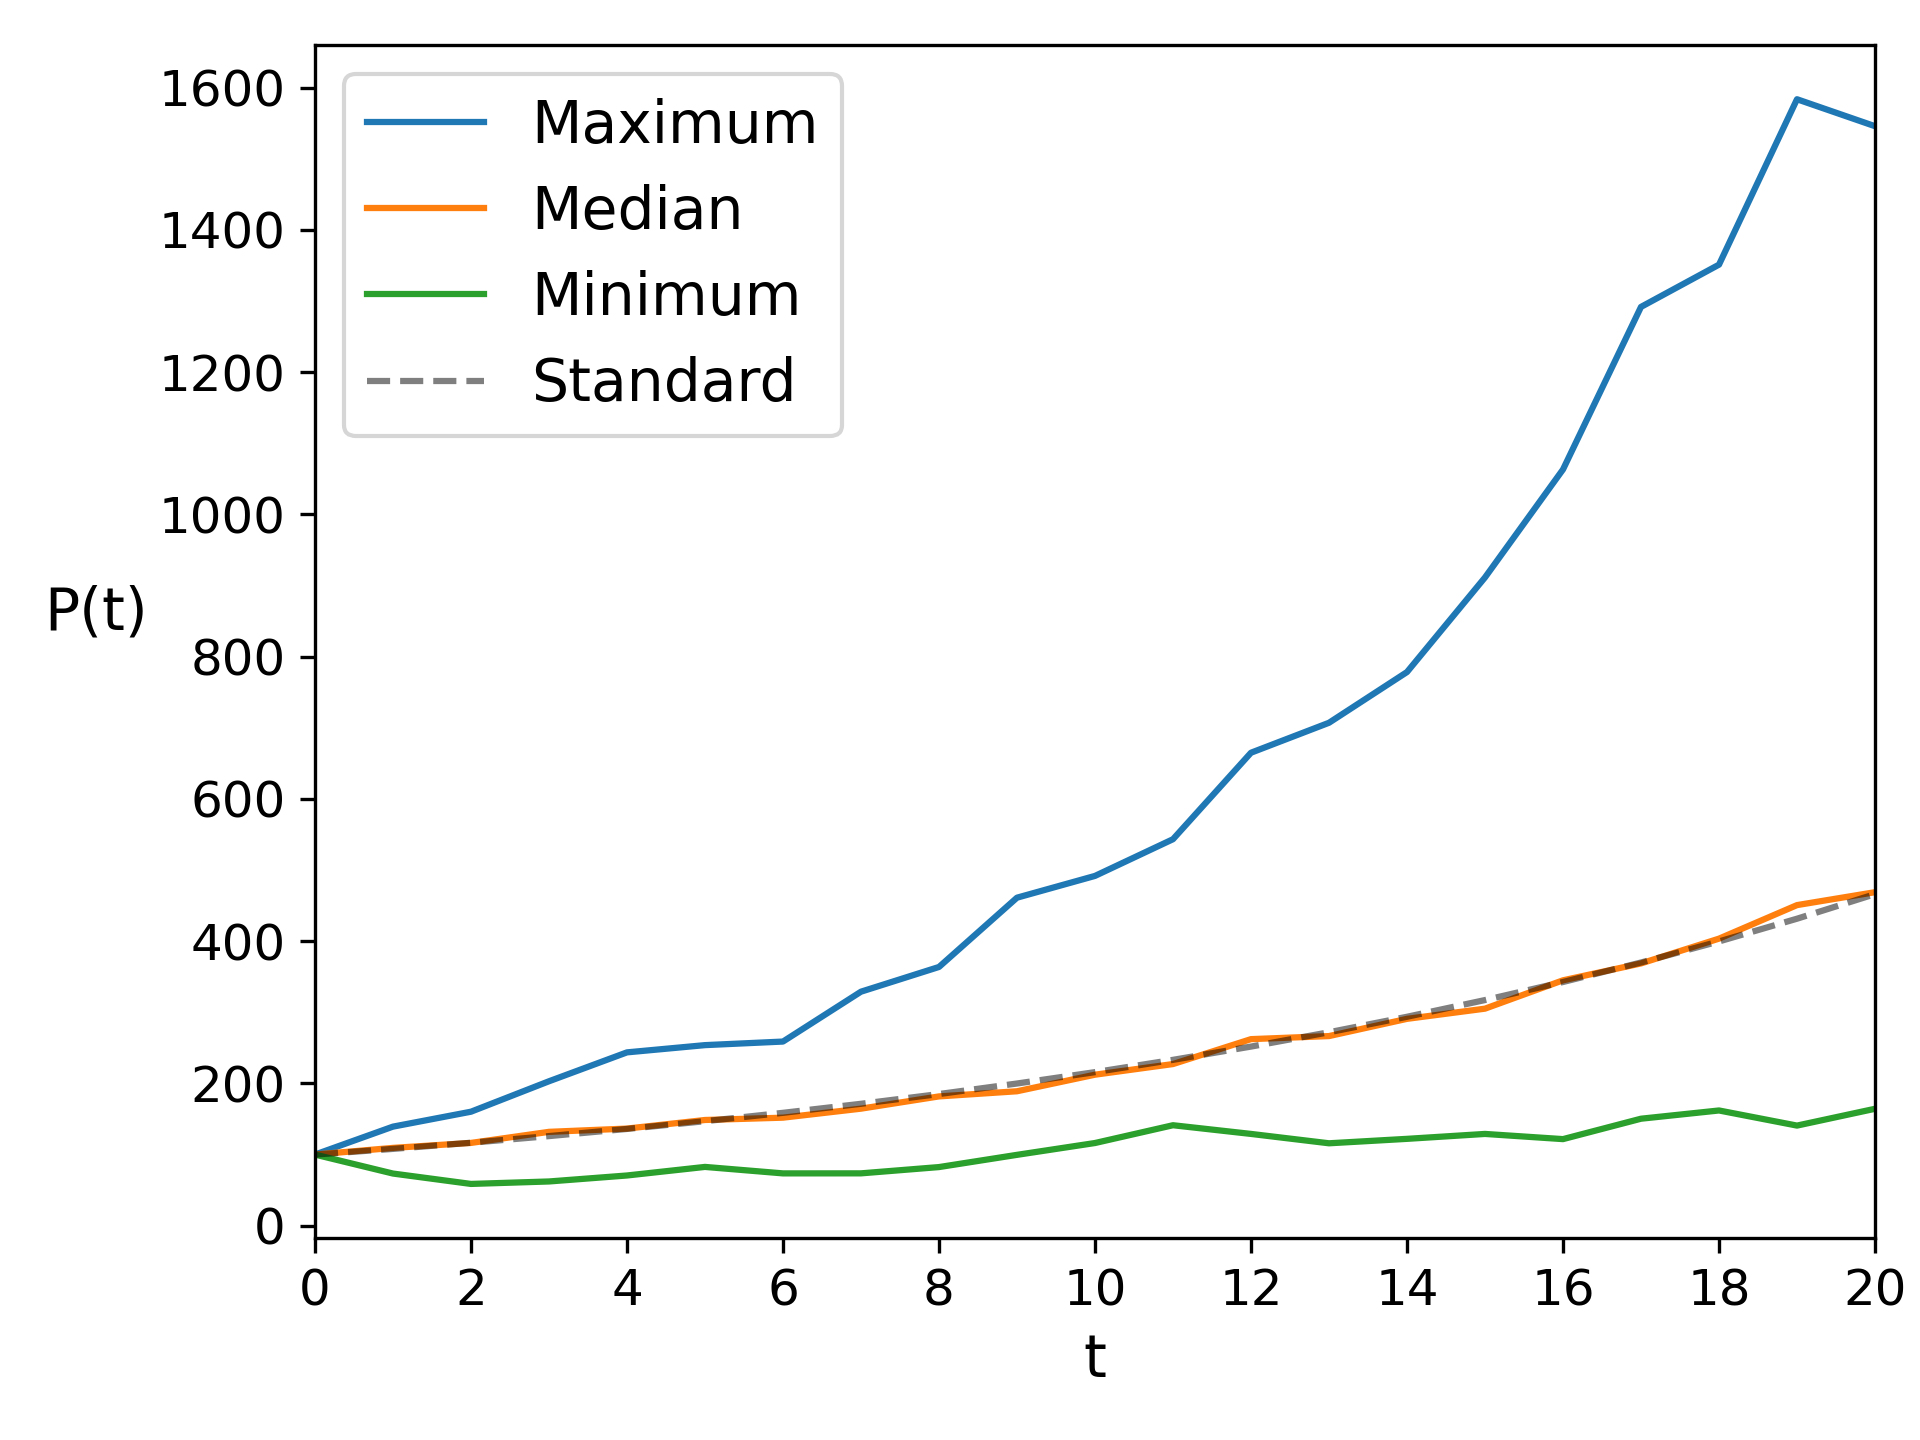
\includegraphics[width=.95\linewidth]{./plots/demographic.png}
        \caption{$b = \mathcal{N}(0.4,0.1)$ and $s = \mathcal{N}(0.68, 0.07)$}
        \label{fig:demographic-standard}
    \end{subfigure}%
    \begin{subfigure}{.5\textwidth}
        \centering
        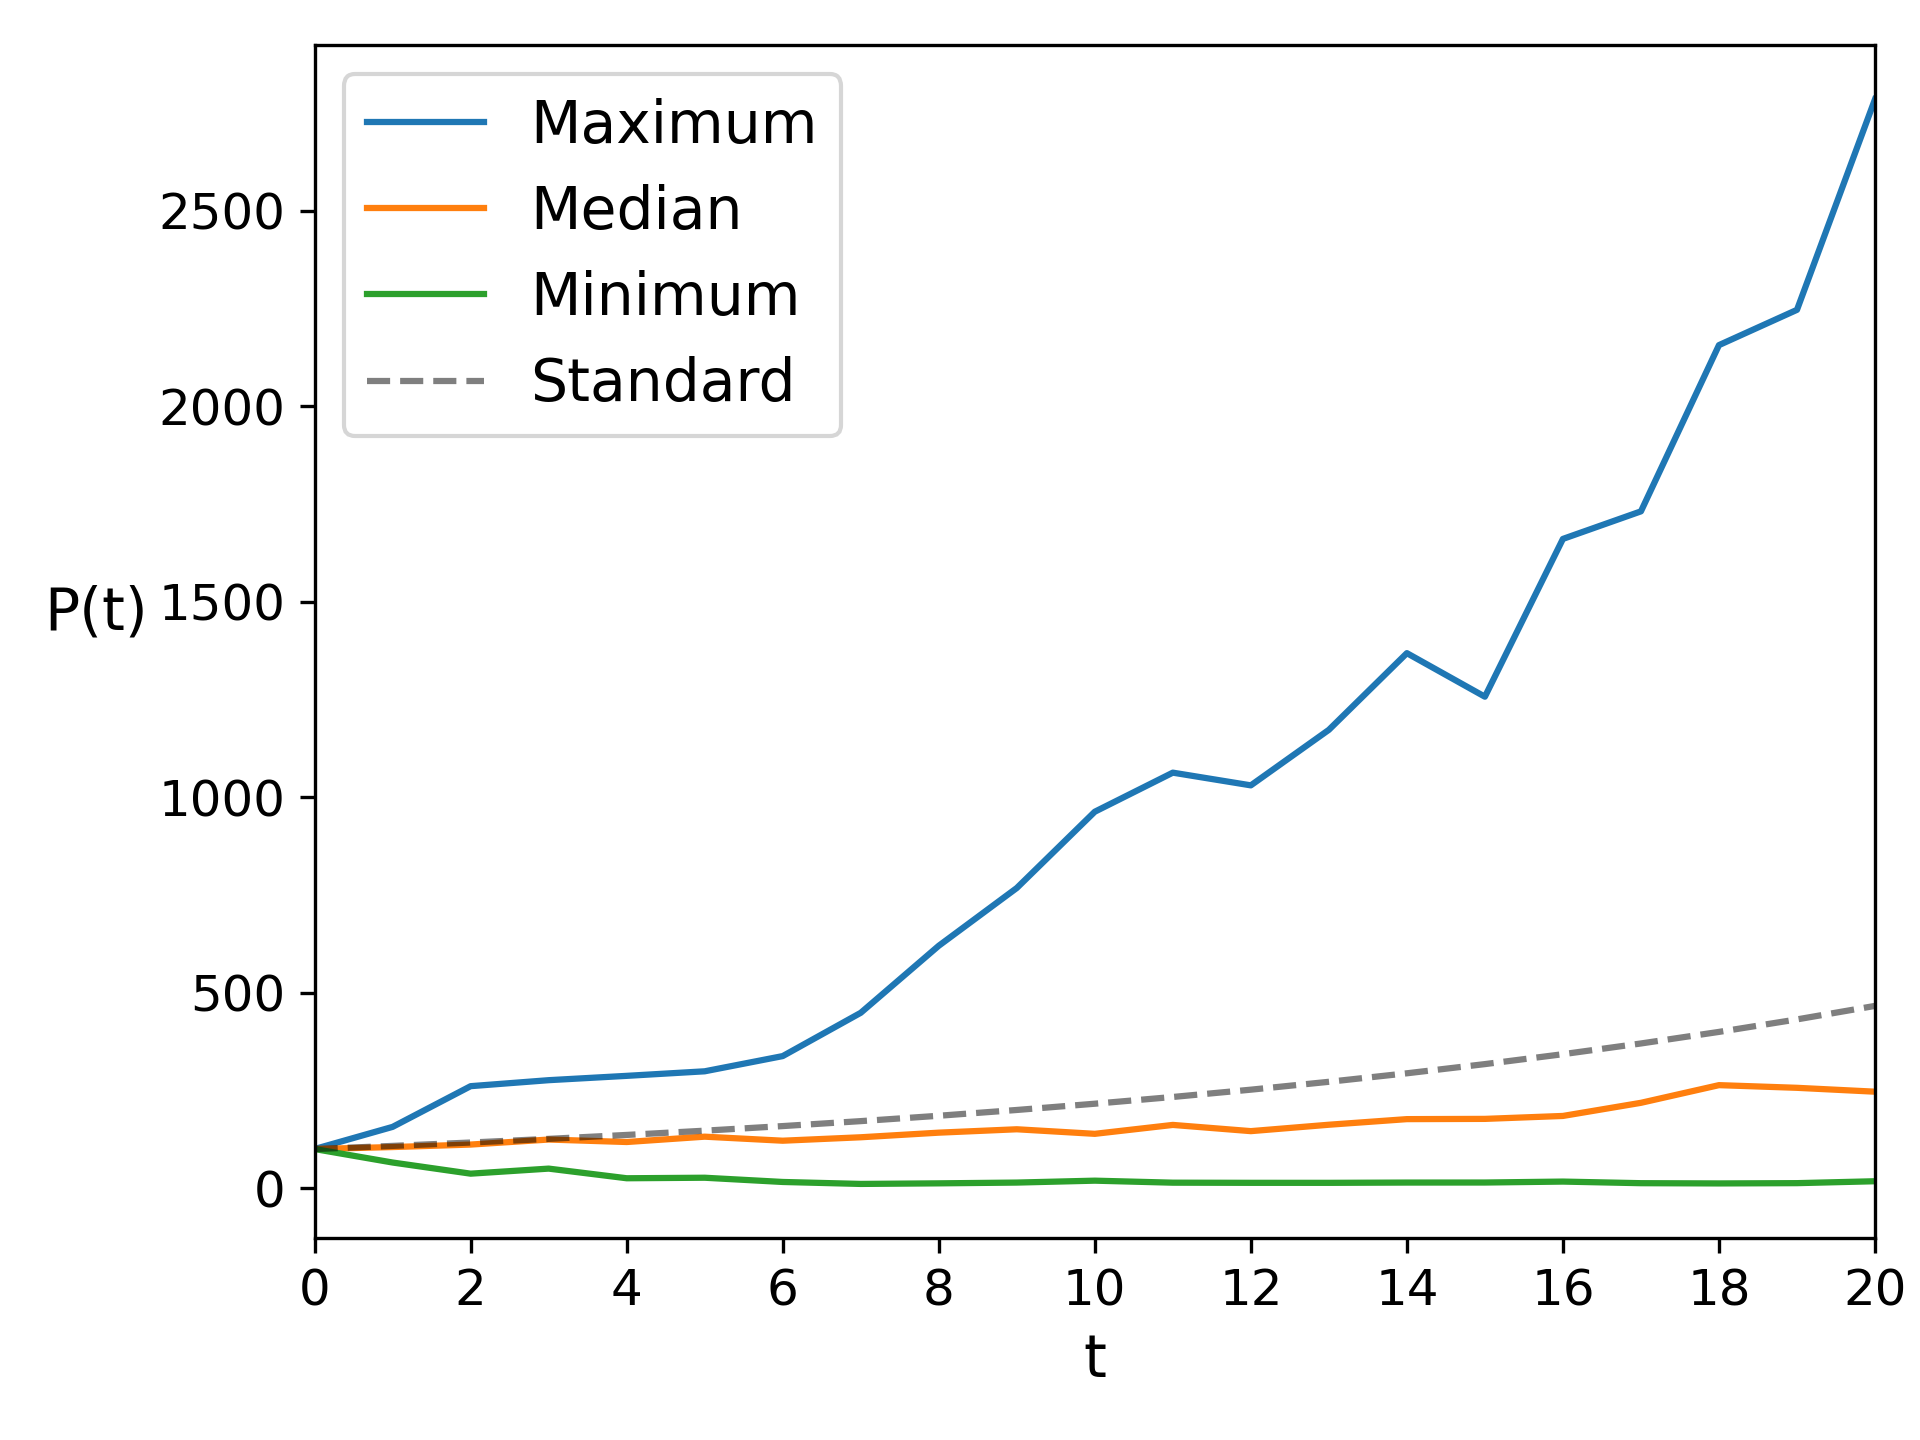
\includegraphics[width=.95\linewidth]{./plots/demographic_higher_dev.png}
        \caption{$b = \mathcal{N}(0.4,0.2)$ and $s = \mathcal{N}(0.68, 0.14)$}
        \label{fig:demographic-higher}
    \end{subfigure}
    \caption{Bobcat population over 20 years and 50 trail runs using different normal distributions for $b$ and $s$ parameters, with the standard exponential function as shown in \cref{fig:exponential} in gray.}
    \label{fig:demographic}
\end{figure}

In \cref{fig:demographic-standard} we see that our median stays fairly close to our initial exponential function. The maximum population function varies heavily from our median, while our minimum stays fairly close. This makes sense, our most common values will be in a single standard deviation, in birth rate this will be $0.4 \pm 0.1$, and in survival rate this will be $0.68 \pm 0.07$. Combining this into our $r + 1$ value from \cref{eq:exponential-basic}, we get $1.08 \pm 0.122$. This $0.122$ comes from converting the two standard deviations into a single normal distribution, $\sqrt{0.1^2+0.07^2} \approx 0.122$. We must do this since the randomness in each normal distribution is independent of each other, while the variance will always be constant. So within one standard deviation $r$ will be between $0.202$ and $-0.042$. Thus, we will tend to have between a larger positive growth rate and a smaller negative growth rate. So, when we are on the positive side of our standard deviation we will grow more than when we are on the negative side of our standard deviation.

This model is quite sensitive to a change in this deviation, if we double the previous deviations, as we see in \cref{fig:demographic-higher}, our maximum goes significantly higher than before. This now changes our first deviation to have a birth rate $0.4 \pm 0.2$ and a survival rate $0.68 \pm 0.14$, or $r$ to be between $0.324$ and $-0.164$. With both a larger positive and negative growth rate we see our maximum grow faster, and our minimum approach zero, which it had not before in \cref{fig:demographic}.

One major change we see is that the median trends below the standard exponential function. This makes sense though, the median represents the ``middle of the road'' population. Say we have a very good year, a growth rate of $1.42$, followed by a very bad year, a growth rate of $0.74$. We know that the growth rates compound over the years, so on the third year we would expect $1.42 \times 0.74 \times P(t-2)$, or a growth of $5.08\%$. While, our standard model with a fixed growth rate will have $1.08 \times 1.08 \times P(t-2)$, or a growth of $16.64\%$. In our previous model we would get $1.25 \times 0.91 \times P(t-1)$, or a growth of $13.75\%$. Thus, as our standard deviation grows, our median gets further, and in our case further negative, from the exponential model.


\section{Environmental Stochasticity}

\begin{figure}[b]
    \centering
    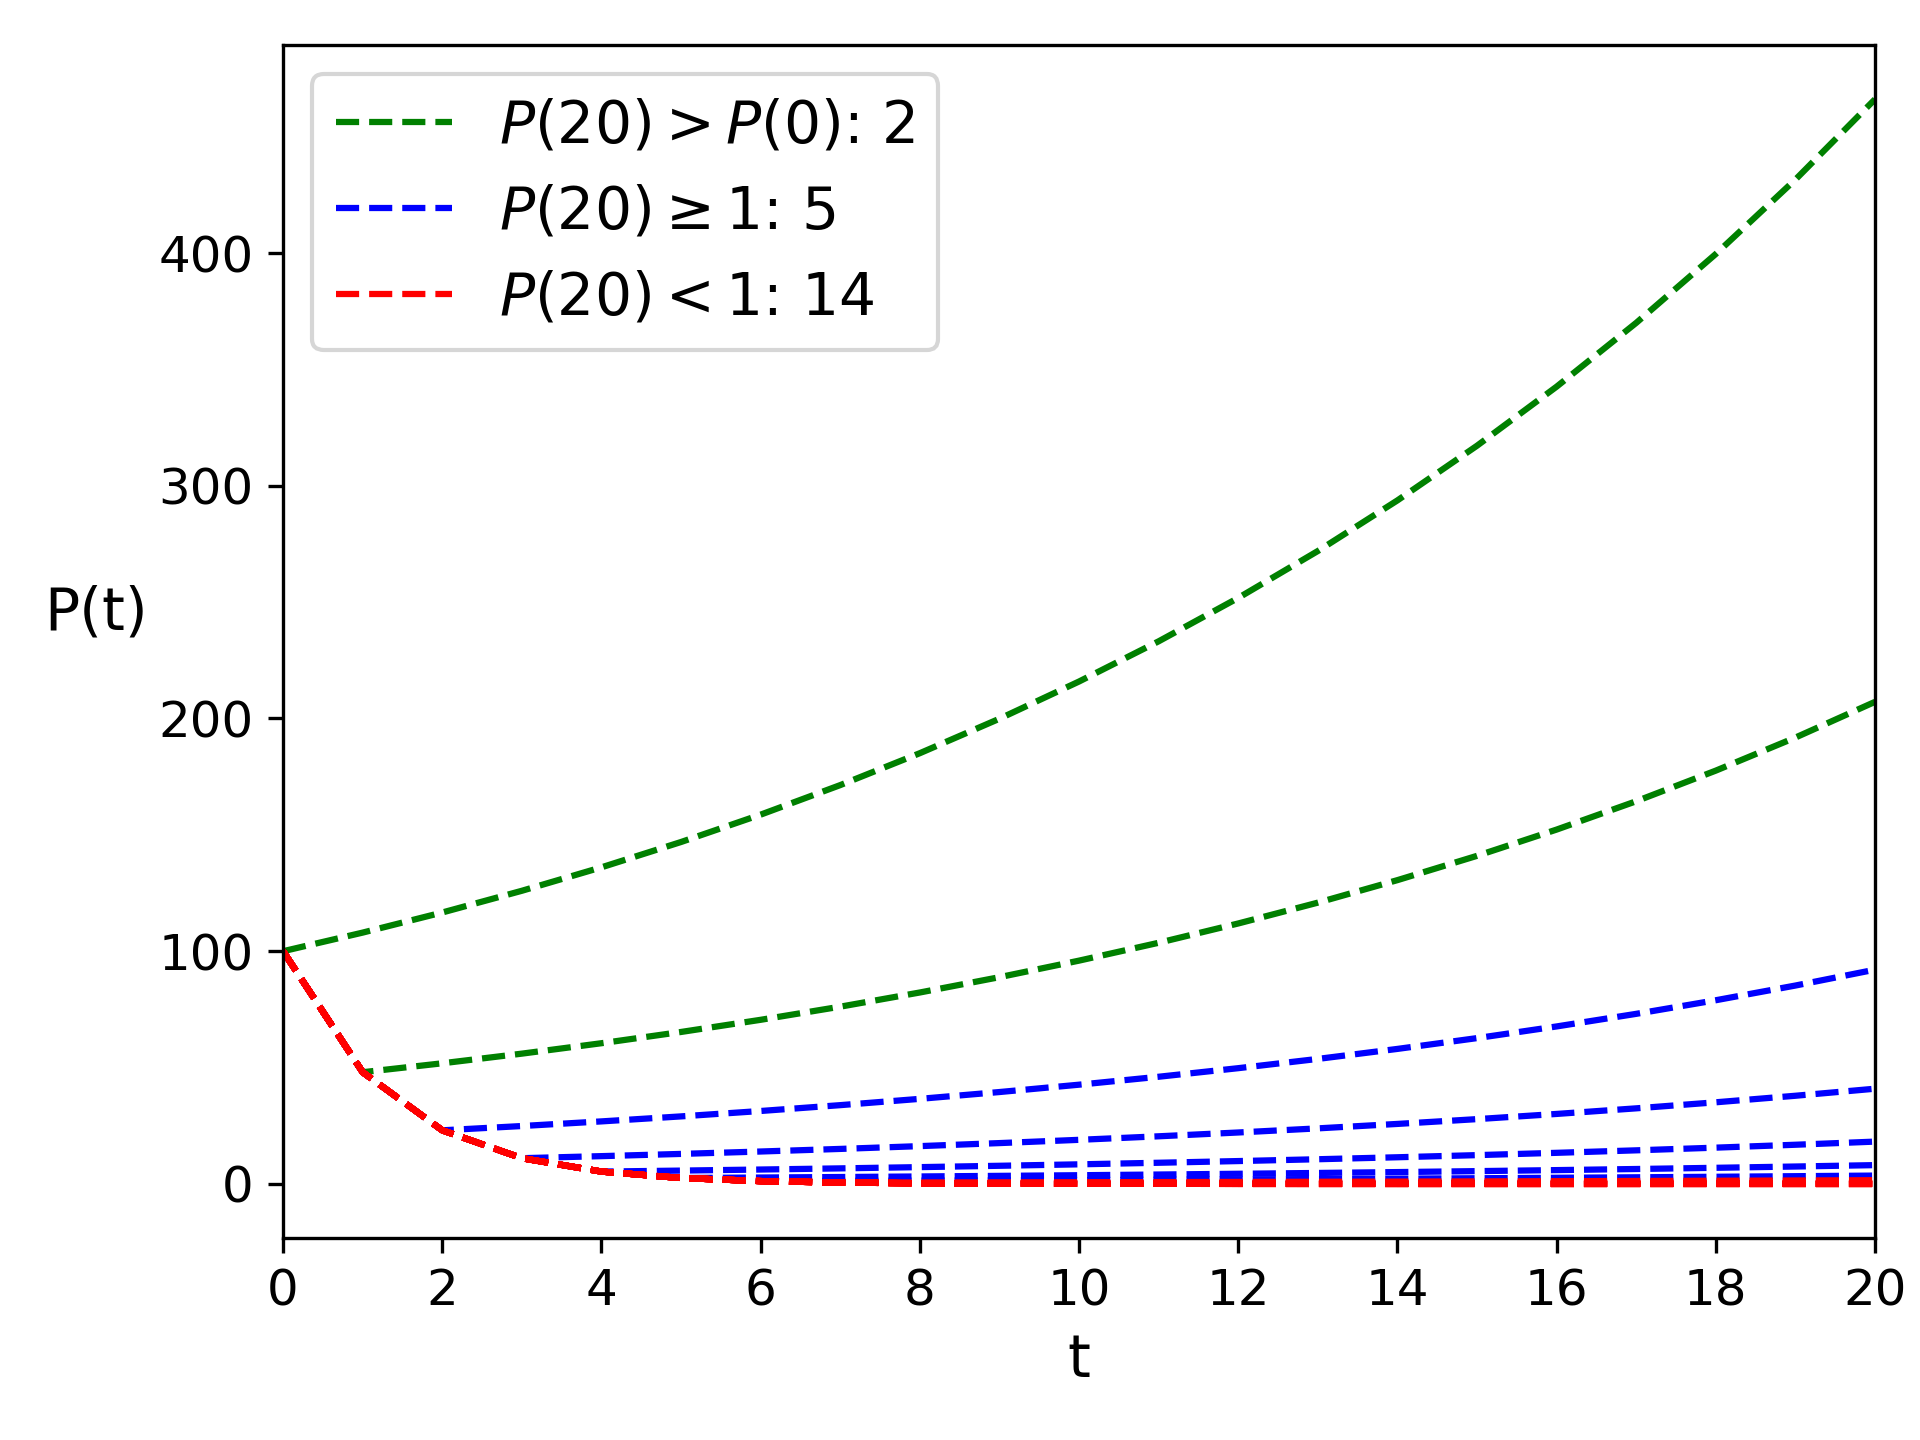
\includegraphics[width=.5\linewidth]{plots/environmental_classes.png}
    \caption{Possible environmental results for all $\sigma(t)$ values in \cref{eq:environmental-piecewise}. Using $b = 0.4$ and $s = 0.68$, and $b = 0.1$, $s = 0.38$ during a catastrophe.}
    \label{fig:environmental-classes}
\end{figure}

In the last section we discussed a model which mimicked variability within a bobcat population's birth and survival rates. This change is usually looked at as internal and varies regularly without one finite cause. In this section we look at the external, or environmental, impact on birth and survival rates.

In order to demonstrate this we introduce a catastrophe, which happens on average once every twelve years. One difference from demographic stochasticity is these `events' will impact birth and survival rates in the same manner. In our example, a catastrophe will reduce both birth and survival rates by 30\%, while our demographic stochasticity model could reduce the survival rates but increase the birth rates.

When our catastrophe happens, we know that our basic model simply has a \\$(b-0.3 + s-0.3)=(b+s - 0.6)$ coefficient. If we define a function $\tau(t)$, which has equal probability of producing any integer from 1 to 12. We can then write our population as a piecewise recurrence.

\begin{equation} \label{eq:environmental-piecewise}
    P(t)=\begin{cases}
        (b+s)P(t-1) & \text{if } \tau(t) > 1 \\
        (b+s-0.6)P(t-1) & \text{if } \tau(t) = 1
    \end{cases}
\end{equation}

\Cref{eq:environmental-piecewise} can be solved by evaluating the two pieces if we assume a constant $\tau(t)$, first we have our standard exponential $P(t)=(b+s)^tP(0)$, then our catastrophe exponential $P(t)=(b+s-0.6)^tP(0)$. If we introduce a function $\sigma(t)$, being the number of times a catastrophe happens over $t$ years. We can create one exponential function.

\begin{equation} \label{eq:environmental-exponential}
    P(t) = (b+s-0.6)^{\sigma(t)}(b+s)^{t-\sigma(t)}P(0)
\end{equation}

Notice that in \cref{eq:environmental-exponential} $P(t)$ changes based off $\sigma(t)$, i.e. the total number of catastrophes, and not when those catastrophes happen. This means that for $P(20)$, there can be 21 possible functions, where $\sigma(t) = 0 \lor 1 \lor \ldots \lor 20$. We see this behavior in \cref{fig:environmental-classes}. We can also see that if we have either $0$ or $1$ catastrophe (the green lines) we will end up growing larger than the initial population. If $1 < \sigma(t) < 7$ (the blue lines), our population will not fall below $1$, i.e. the population will not die off. For any $7 \le \sigma(t)$ (the red lines), our population will die off. This gives us a general idea of what will happen in a maximum and minimum situation, the uppermost green line being our maximum, when no catastrophes happen, the lowest red line being the worst case where 20 catastrophes happen, which will be similar results for if we have 7 or more catastrophes.

\begin{figure}[h!]
    \centering
    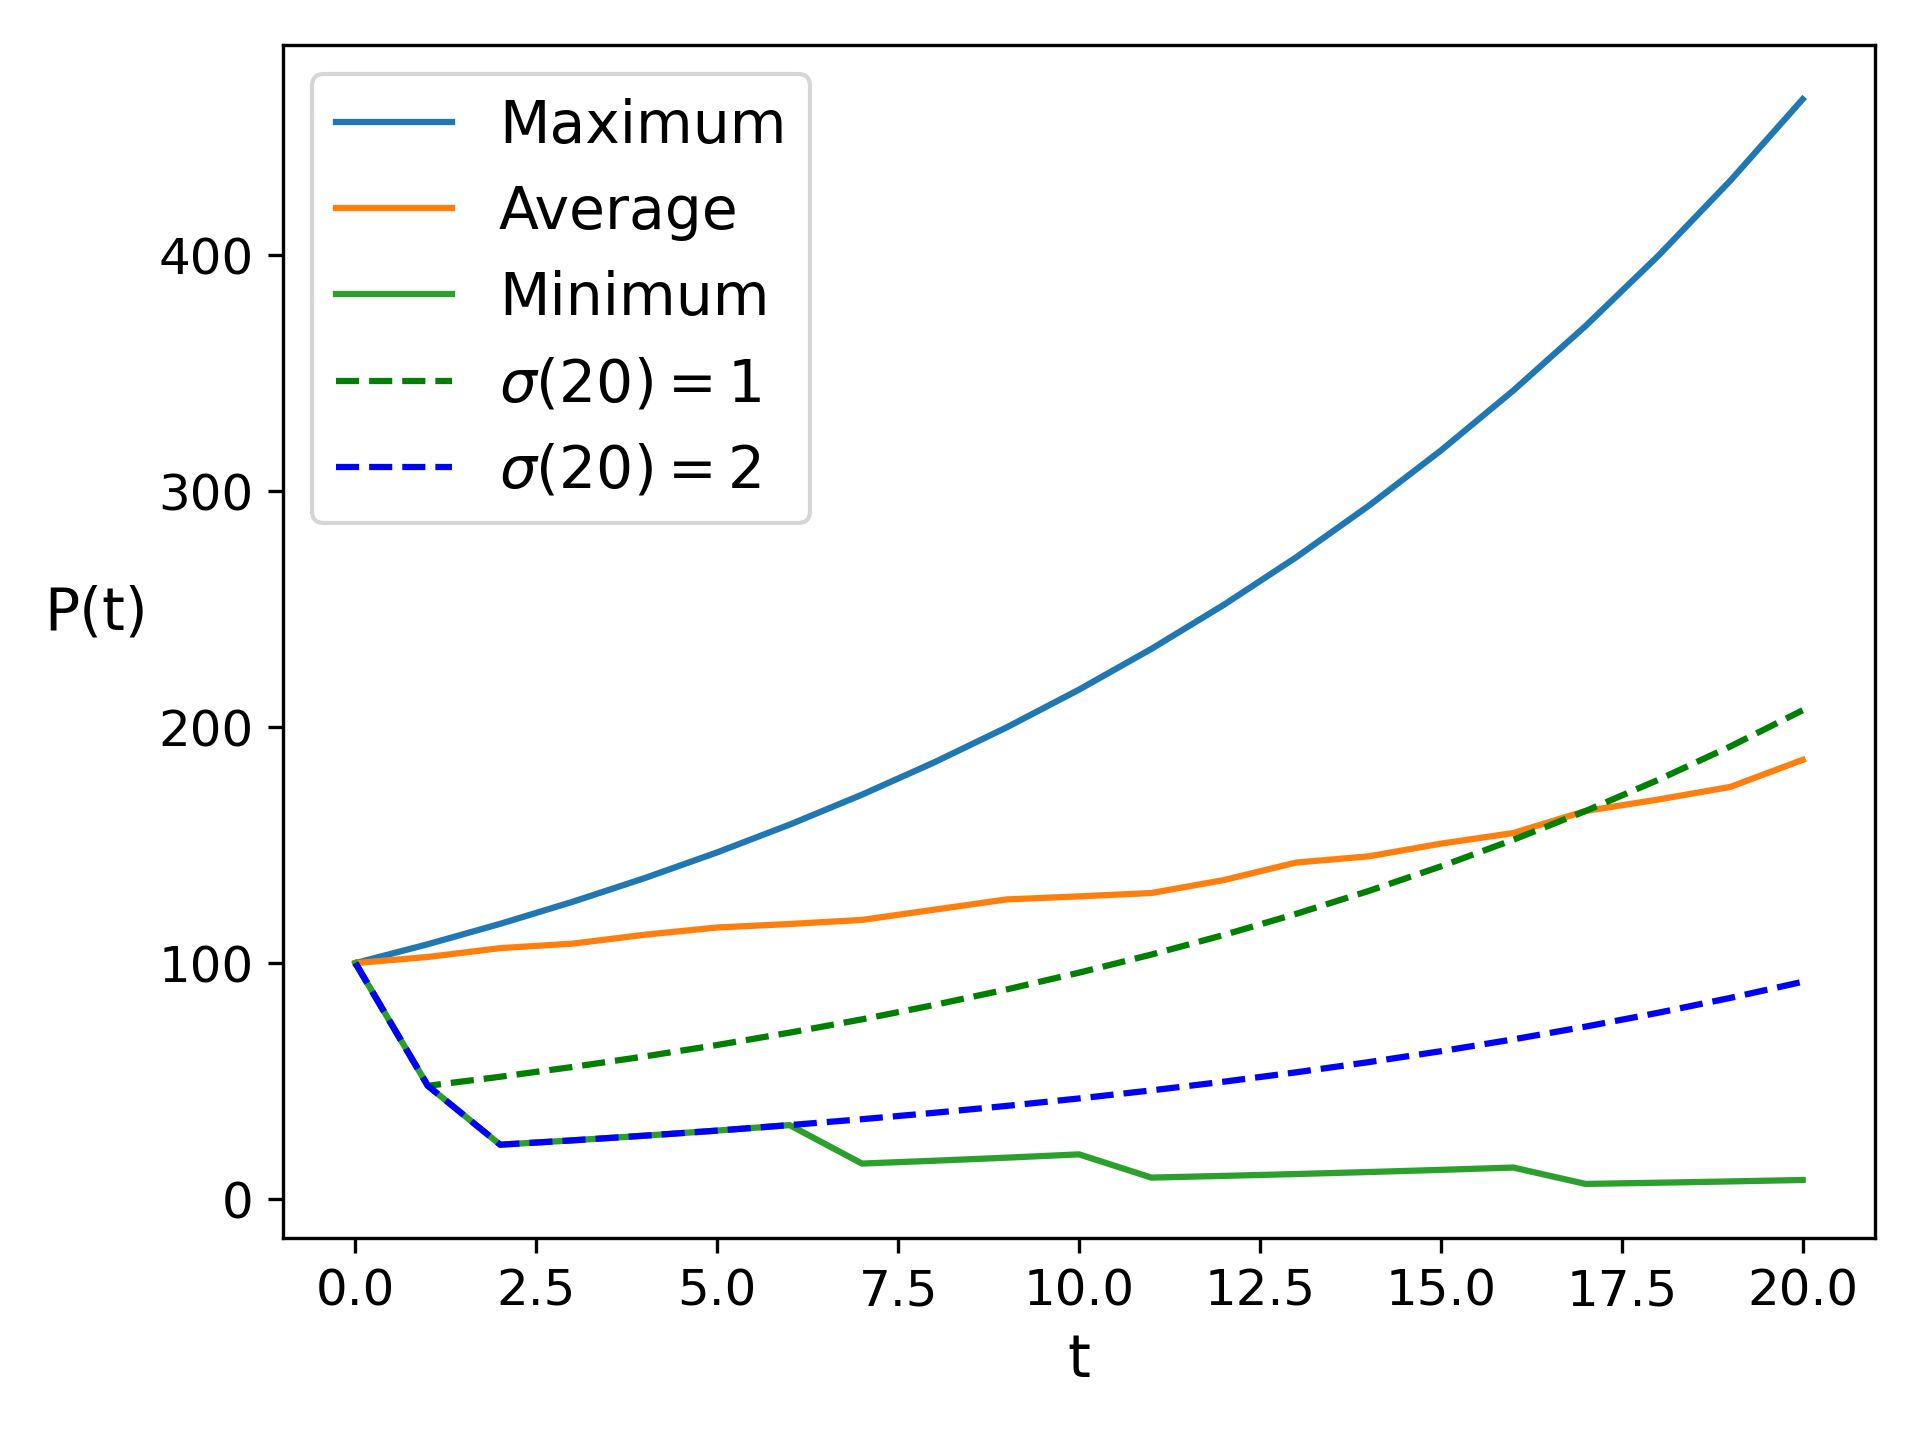
\includegraphics[width=.5\linewidth]{plots/environmental.png}
    \caption{50 trials of environment model with $\frac{1}{12}$ odds of a catastrophe. Using $b = 0.4$ and $s = 0.68$, and $b = 0.1$, $s = 0.38$ during a catastrophe.}
    \label{fig:environmental}
\end{figure}

In average cases we can break down the likelihood of these maximum and minimum situations. Since we know that $\tau(t)$ has exactly $\frac{1}{12}$ odds of having a catastrophe, we can calculate these odds. The likelihood of no catastrophe happening in a single year is $1 - \frac{1}{12}$ or $\frac{11}{12}$, thus over twenty years we have a $\left(\frac{11}{12}\right)^{20}$ chance of this happening, or roughly $17.55\%$ chance of no catastrophe occurring. To find when a specific number of events occur we need to use a combinatorial function, known as the binomial coefficient, to find all possible ways a catastrophe could occur over 20 years. This is denoted $\binom{20}{c}$, where $c$ is the number of catastrophes. Then we multiply by the odds of the number of catastrophes in a row, $\frac{1}{12}^c \cdot \frac{11}{12}^{20-c}$. We see a generalized form of this in \cref{eq:environmental-catastrophe-rate}, where $\lambda$ is the odds of the amount of catastrophes $c$ happening at a catastrophe rate of $c_r$. If we sum this result over the amount we want, i.e. 7 to 20, $\sum_{c=7}^{20}\left(\binom{20}{c} \cdot \frac{1}{12}^c \frac{11}{12}^{20-c}\right)$, we can get the exact percentage of being in the case where our population dies off. Computing this gives that there is roughly $0.0815\%$ chance of this occurring, which is dwarfed by the chances of no catastrophes happening. Doing this same computation (or by process of elimination) we find a $82.37\%$ of us having 1 to 6 catastrophes, or a $99.92\%$ chance of having 0 to 6 catastrophes. Thus, percentage wise it is significantly more likely for our population to not die off than to die off.

\begin{equation} \label{eq:environmental-catastrophe-rate}
    \lambda(c, c_r) = \binom{20}{c} c_r^c (1-c_r)^{20-c}
\end{equation}

\Cref{fig:environmental} shows us what happens in an average case (the orange line), along with the expected minimums and maximums. Using \cref{eq:environmental-catastrophe-rate} summed for 1 to 2 catastrophes, we find that we will be in this range $59.46\%$ of the time, and $31.9\%$ we will have exactly 1 catastrophe while $27.55\%$ of the time we will have exactly 2, thus the average is between these and tends to be closer to 1 catastrophe.

\begin{figure}[h!]
    \centering
    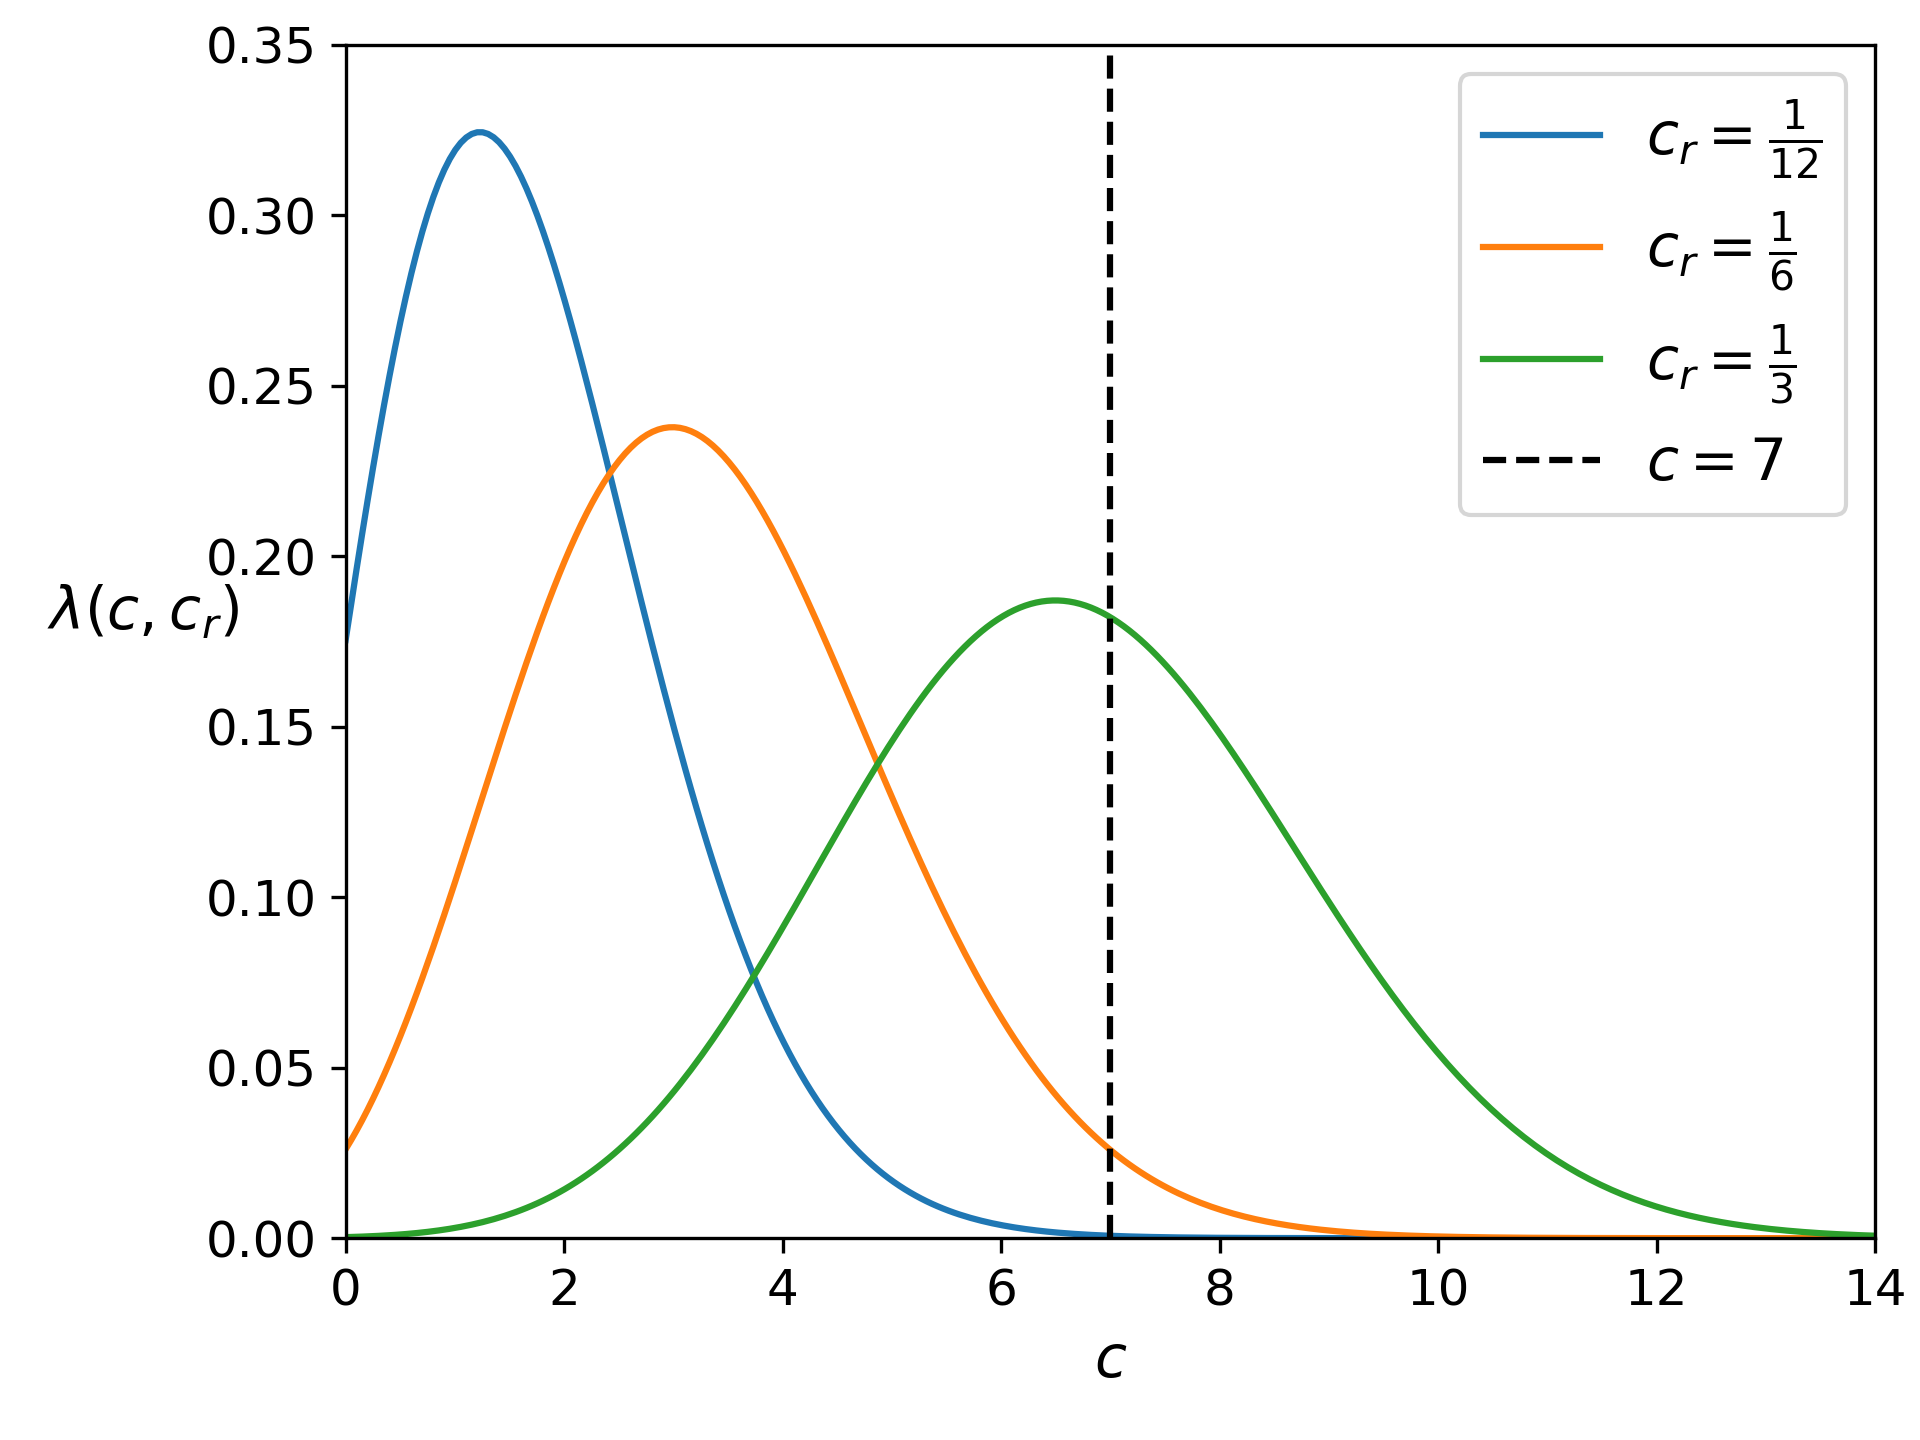
\includegraphics[width=.5\linewidth]{plots/catastrophe_rate.png}
    \caption{Plots of \cref{eq:environmental-catastrophe-rate} with differing $c_r$ values.}
    \label{fig:environmental-catastrophe-rate}
\end{figure}

The model is only slightly sensitive to changes in catastrophe rate. As we see in \cref{fig:environmental-catastrophe-rate} as we increase the odds of a catastrophe we have higher odds of 7 or more catastrophes, leading to a zero population. However, this means there are many rates we can use that will only slightly decrease average final population over 20 years. This model is, on average, much more predictable than the demographic model. This model is also significantly less sensitive to parameter changes. We also know this model directly effects the average final population, while the previous model's average will always stay near the basic model, regardless of how we implement our normal distribution.

\section{Conclusion}

In this paper we discussed two different stochastic methods of modeling. We focused our models around a basic exponential model, then used either demographic or environmental stochasticity. We analyzed how we can use normal distributions to vary parameters of the exponential model, and how the standard deviations play a role in the outcome of the model. For environmental stochasticity we analyzed the combinatorics behind a fairly simple random percentage reduction of parameters. Ultimately, these methods can be expanded to more complex models to add realism.

\end{document}